\chapter{PHÂN TÍCH YÊU CẦU VÀ THIẾT KẾ HỆ THỐNG}
\label{ch:thietke}

\vspace{0.5cm}
\noindent\textit{Chương này chuyển các cơ sở lý thuyết ở Chương 2 thành thiết kế cụ thể cho hệ thống của đồ án. Nội dung được trình bày theo luồng dữ liệu từ thiết bị Zigbee, qua Gateway và Message Queuing Telemetry Transport (MQTT), tới Cloud Backend, cơ sở dữ liệu và Mobile App. Cách sắp xếp này giúp người đọc xác định rõ dữ liệu bắt đầu ở đâu, được xử lý bởi thành phần nào và kết thúc tại đâu.}
\vspace{0.5cm}

\section{Phạm vi và giả định thiết kế}
\label{sec:ch3-scope}

Hệ thống được thiết kế cho mô hình thử nghiệm trong một phòng hoặc phòng thí nghiệm. Phiên bản hiện tại quản lý một Gateway và ba loại thiết bị chính gồm đèn, công tắc và cảm biến chuyển động. Trong mô hình dữ liệu, ba loại thiết bị này lần lượt có giá trị \texttt{light}, \texttt{switch} và \texttt{motion}. Giá trị \texttt{occupancy} biểu diễn trạng thái phát hiện hiện diện của cảm biến chuyển động, không phải một loại thiết bị độc lập.

Thiết bị Zigbee không giao tiếp trực tiếp với Internet. Gateway đặt tại mạng cục bộ duy trì kết nối với bộ xử lý mạng EFR32, chuyển dữ liệu Zigbee thành bản tin MQTT và thực hiện chiều ngược lại đối với lệnh điều khiển. Cloud Backend cung cấp giao diện cho Mobile App, lưu dữ liệu bền vững và kiểm soát quyền truy cập. Mobile App là lớp tương tác với người dùng, không kết nối trực tiếp tới thiết bị hoặc Gateway.

Với phạm vi này, Zigbee được chọn làm mạng thiết bị cục bộ vì hệ thống cần các node công suất thấp, trao đổi bản tin nhỏ và có khả năng mở rộng theo mesh. Các công nghệ như Wi-Fi, Thread, LoRaWAN hoặc Matter có ưu điểm riêng, nhưng sẽ làm thay đổi mục tiêu triển khai: Wi-Fi thiên về thiết bị IP trực tiếp, Thread cần stack và Border Router khác, LoRaWAN phù hợp hơn với phạm vi xa, còn Matter chủ yếu giải quyết interoperability ở lớp ứng dụng. Do đó, thiết kế của đồ án tập trung vào việc chứng minh luồng end-to-end Zigbee--Gateway--MQTT--Cloud/App thay vì khảo sát nhiều runtime thiết bị cùng lúc.

\section{Phân tích yêu cầu hệ thống}
\label{sec:ch3-requirements}

\subsection{Tác nhân sử dụng hệ thống}

Hệ thống có ba nhóm tác nhân. Người quản trị quản lý người dùng, thiết bị và quá trình thêm thiết bị. Người dùng điều khiển có thể xem và điều khiển thiết bị trong nhà được gán. Người xem chỉ được quan sát trạng thái và lịch sử sự kiện. Ngoài tác nhân con người, Gateway và các thiết bị Zigbee là tác nhân kỹ thuật vì chúng chủ động gửi trạng thái, sự kiện và phản hồi lệnh.

\subsection{Yêu cầu chức năng}

Bảng \ref{tab:ch3-functional-requirements} tóm tắt các yêu cầu chức năng theo luồng vận hành của hệ thống.

\begin{table}[H]
\centering
\caption{Các yêu cầu chức năng chính}
\label{tab:ch3-functional-requirements}
\small
\begin{tabular}{|>{\centering\arraybackslash}p{1.4cm}|>{\raggedright\arraybackslash}p{4.5cm}|>{\raggedright\arraybackslash}p{8.0cm}|}
\hline
\textbf{Mã} & \textbf{Yêu cầu} & \textbf{Mô tả} \\ \hline
FR-01 & Quản lý mạng Zigbee & Gateway cho phép mở hoặc đóng mạng, nhận thiết bị tham gia và lưu thông tin nhận dạng thiết bị. \\ \hline
FR-02 & Giám sát thiết bị & Hệ thống hiển thị danh sách thiết bị, trạng thái gần nhất và tình trạng trực tuyến. \\ \hline
FR-03 & Điều khiển đèn & Người dùng có quyền gửi lệnh bật hoặc tắt đèn và theo dõi vòng đời của lệnh. \\ \hline
FR-04 & Ghi nhận sự kiện & Công tắc, cảm biến chuyển động và Gateway có thể phát sinh sự kiện để Cloud lưu và hiển thị. \\ \hline
FR-05 & Tự động hóa & Người dùng có quyền tạo và bật/tắt luật tự động hóa dựa trên sự kiện của thiết bị. \\ \hline
FR-06 & Xác thực và phân quyền & Hệ thống xác thực người dùng, duy trì phiên đăng nhập và giới hạn thao tác theo vai trò và phạm vi nhà. \\ \hline
FR-07 & Thêm thiết bị & Người dùng có quyền tạo phiên thêm thiết bị và theo dõi trạng thái của phiên. \\ \hline
\end{tabular}
\end{table}

Các yêu cầu trên tạo thành một vòng kín: thiết bị tham gia mạng, gửi dữ liệu, nhận lệnh và phản hồi; Cloud lưu lại diễn biến; Mobile App cung cấp điểm thao tác cho người dùng.

\subsection{Yêu cầu phi chức năng}

Hệ thống cần tách biệt rõ trách nhiệm giữa các lớp để lỗi ở một lớp không làm thay đổi hợp đồng dữ liệu của lớp khác. Bản tin phải có định danh thiết bị và thời điểm phát sinh. Lệnh điều khiển cần có trạng thái \texttt{accepted}, \texttt{executed}, \texttt{failed} hoặc \texttt{timeout} để người dùng không nhầm việc Cloud nhận yêu cầu với việc thiết bị đã thực thi.

Về bảo mật, Cloud phải từ chối yêu cầu không có phiên hợp lệ và kiểm tra phạm vi truy cập trước khi trả dữ liệu hoặc gửi lệnh. Về khả năng bảo trì, các module Gateway, router Cloud và repository của Mobile App cần có ranh giới rõ. Về kiểm thử, phần mềm Cloud và Mobile App phải có thể chạy test độc lập với phần cứng; các test xuyên suốt cần dùng thiết bị thật và lưu evidence.

\section{Kiến trúc tổng thể hệ thống}
\label{sec:ch3-architecture}

Hình \ref{fig:ch3-system-architecture} trình bày các lớp chính và hai chiều dữ liệu của hệ thống.

\begin{figure}[H]
\centering
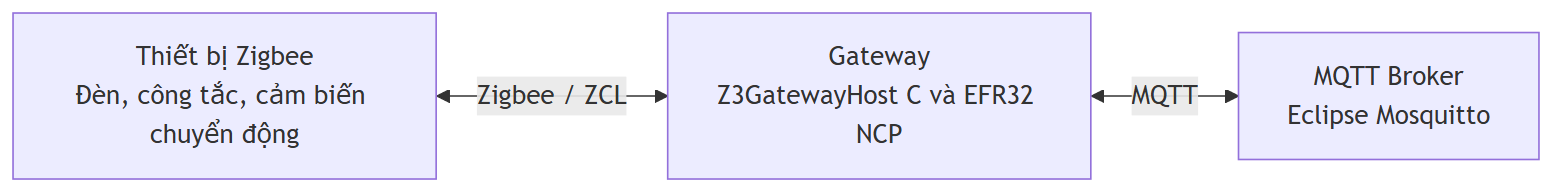
\includegraphics[width=0.86\textwidth]{Images/mermaid/ch3_system_architecture_local.png}\\[0.25cm]
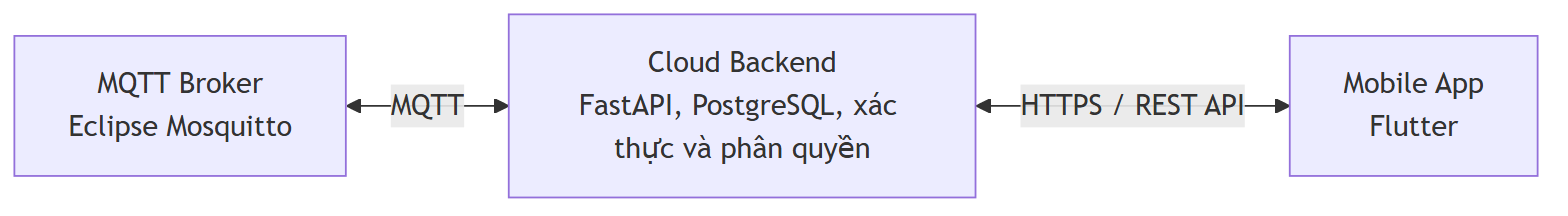
\includegraphics[width=0.82\textwidth]{Images/mermaid/ch3_system_architecture_cloud.png}
\caption{Kiến trúc tổng thể và đường truyền dữ liệu của hệ thống}
\label{fig:ch3-system-architecture}
\end{figure}

Theo chiều đi lên, thiết bị gửi trạng thái hoặc sự kiện qua mạng Zigbee. Gateway chuẩn hóa dữ liệu thành bản tin MQTT, Cloud kiểm tra và lưu vào cơ sở dữ liệu, sau đó Mobile App đọc dữ liệu qua Application Programming Interface (API). Theo chiều đi xuống, Mobile App gửi yêu cầu tới Cloud; Cloud tạo bản ghi lệnh, phát bản tin MQTT; Gateway chuyển lệnh thành thao tác Zigbee và gửi phản hồi về Cloud.

\section{Thiết kế thiết bị và trạng thái}
\label{sec:ch3-device-model}

\subsection{Mô hình thiết bị}

Bảng \ref{tab:ch3-device-types} mô tả hợp đồng tối thiểu của từng loại thiết bị. Mô hình này giúp Cloud và Mobile App xử lý thiết bị theo loại mà không cần hiểu chi tiết firmware.

\begin{table}[H]
\centering
\caption{Mô hình các loại thiết bị phiên bản hiện tại}
\label{tab:ch3-device-types}
\small
\begin{tabular}{|>{\raggedright\arraybackslash}p{2.3cm}|>{\raggedright\arraybackslash}p{3.2cm}|>{\raggedright\arraybackslash}p{4.2cm}|>{\raggedright\arraybackslash}p{4.2cm}|}
\hline
\textbf{Loại} & \textbf{Vai trò Zigbee} & \textbf{Trạng thái chính} & \textbf{Hành vi chính} \\ \hline
\texttt{light} & Router, On/Off Server & \texttt{power}, \texttt{level}, \texttt{reachable} & Nhận lệnh bật/tắt và báo cáo trạng thái. \\ \hline
\texttt{switch} & Router, On/Off Client & \texttt{reachable}, tùy chọn \texttt{battery} & Phát sinh sự kiện khi người dùng nhấn nút. \\ \hline
\texttt{motion} & End Device, Occupancy Sensing Server & \texttt{occupancy}, \texttt{reachable}, tùy chọn \texttt{battery} & Báo sự kiện khi trạng thái hiện diện thay đổi. \\ \hline
\end{tabular}
\end{table}

Định danh EUI-64 được dùng để liên hệ thiết bị vật lý với bản ghi logic trong hệ thống. Địa chỉ mạng ngắn chỉ có ý nghĩa trong phiên mạng hiện tại, vì vậy không được dùng làm định danh bền vững.

\subsection{Trạng thái, sự kiện và lệnh}

Trạng thái mô tả giá trị hiện tại của thiết bị, ví dụ đèn đang bật. Sự kiện mô tả một việc vừa xảy ra, ví dụ công tắc được nhấn hoặc cảm biến thay đổi giá trị hiện diện. Lệnh mô tả yêu cầu thay đổi trạng thái, ví dụ bật đèn. Việc tách ba khái niệm này giúp hệ thống tránh dùng một bản ghi cho nhiều mục đích.

\section{Luồng dữ liệu hệ thống}
\label{sec:ch3-data-flow}

\subsection{Luồng đi lên: thiết bị báo cáo lên Cloud}

Thiết bị gửi báo cáo thuộc tính hoặc sự kiện tới Coordinator. Gateway nhận callback từ Zigbee stack, xác định loại thiết bị, thêm định danh và đóng gói dữ liệu theo hợp đồng MQTT. Cloud nhận bản tin, cập nhật thời điểm nhìn thấy thiết bị, lưu trạng thái hoặc sự kiện và cung cấp dữ liệu cho Mobile App.

\subsection{Luồng đi xuống: người dùng gửi lệnh điều khiển}

Hình \ref{fig:ch3-downlink-flow} mô tả luồng điều khiển đèn ở mức thiết kế.

\begin{figure}[H]
\centering
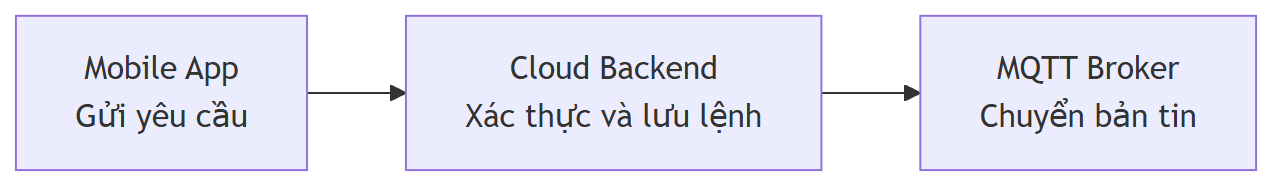
\includegraphics[width=0.76\textwidth]{Images/mermaid/ch3_downlink_request.png}\\[0.25cm]
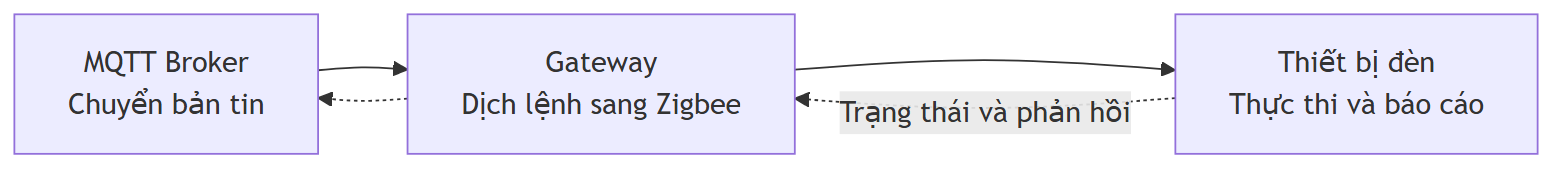
\includegraphics[width=0.76\textwidth]{Images/mermaid/ch3_downlink_execution.png}
\caption{Luồng thiết kế cho lệnh điều khiển đèn}
\label{fig:ch3-downlink-flow}
\end{figure}

Cloud trả trạng thái \texttt{accepted} khi đã nhận và phát lệnh, không đồng nghĩa thiết bị đã thực thi. Mobile App tiếp tục truy vấn trạng thái lệnh. Khi Gateway gửi phản hồi, Cloud cập nhật lệnh thành \texttt{executed} hoặc \texttt{failed}; worker thời gian chờ chuyển lệnh quá hạn thành \texttt{timeout}.

\subsection{Luồng tự động hóa}

Một luật tự động hóa gồm nguồn kích hoạt, điều kiện tùy chọn và hành động. Ví dụ, sự kiện \texttt{occupancy\_changed} của cảm biến chuyển động có thể kích hoạt hành động bật đèn. Cloud quản lý cấu hình luật; Gateway có thể thực hiện luật cục bộ để giảm phụ thuộc vào đường truyền Internet. Sự đánh đổi là luật cần được đồng bộ và có phiên bản để Cloud và Gateway không dùng hai cấu hình khác nhau.

\section{Thiết kế hợp đồng MQTT}
\label{sec:ch3-mqtt-contract}

MQTT topic sử dụng tiền tố \texttt{sb/v1/\{tenant\}/\{site\}/\{gateway\}}. Ba thành phần này tạo không gian tên cho đơn vị sử dụng, địa điểm và Gateway. Payload sử dụng envelope \texttt{sb.v1} để các bên kiểm tra phiên bản hợp đồng.

Bảng \ref{tab:ch3-mqtt-topics} trình bày các nhóm topic chính.

\begin{table}[H]
\centering
\caption{Các nhóm topic MQTT chính}
\label{tab:ch3-mqtt-topics}
\footnotesize
\begin{tabular}{|>{\raggedright\arraybackslash}p{5.3cm}|>{\raggedright\arraybackslash}p{3.3cm}|>{\raggedright\arraybackslash}p{5.0cm}|}
\hline
\textbf{Mẫu topic} & \textbf{Chiều dữ liệu} & \textbf{Mục đích} \\ \hline
\texttt{devices/\{type\}/\{id\}/reported} & Gateway lên Cloud & Báo trạng thái hiện tại. \\ \hline
\texttt{devices/\{type\}/\{id\}/event} & Gateway lên Cloud & Báo sự kiện của thiết bị. \\ \hline
\texttt{devices/\{type\}/\{id\}/registry} & Gateway lên Cloud & Báo định danh và phân loại thiết bị. \\ \hline
\texttt{commands/\{id\}/request} & Cloud xuống Gateway & Yêu cầu thực thi lệnh. \\ \hline
\texttt{commands/\{id\}/reply} & Gateway lên Cloud & Báo kết quả hoặc nguyên nhân lỗi. \\ \hline
\texttt{gateway/online}, \texttt{gateway/health} & Gateway lên Cloud & Báo kết nối và tình trạng Gateway. \\ \hline
\end{tabular}
\end{table}

Việc dùng topic theo thiết bị giúp Cloud đăng ký nhận theo mẫu. Tuy nhiên, quyền truy cập của MQTT Broker phải giới hạn đúng tiền tố tenant, site và gateway để một Gateway không đọc hoặc ghi dữ liệu của Gateway khác.

\section{Thiết kế Gateway biên}
\label{sec:ch3-gateway-design}

Gateway được thiết kế là ứng dụng Host viết bằng C, sử dụng \texttt{libmosquitto} để làm việc với MQTT và giao tiếp với EFR32 NCP qua EmberZNet Serial Protocol (EZSP) trên Asynchronous Serial Host (ASH). Thiết kế này không dùng một tiến trình Python làm cầu nối trung gian.

Callback MQTT chỉ kiểm tra sơ bộ và đưa lệnh vào hàng đợi. Vòng lặp chính lấy lệnh, phân tích envelope, xác định đích, gọi module điều khiển phù hợp và phát phản hồi. Ở chiều ngược lại, callback của Zigbee stack chuyển báo cáo thuộc tính và sự kiện cho module MQTT. Cách dùng hàng đợi tránh thực hiện thao tác Zigbee dài bên trong luồng callback mạng.

Gateway còn duy trì registry thiết bị để ánh xạ EUI-64, địa chỉ mạng và loại thiết bị. Khi thiết bị mới tham gia, Gateway thực hiện discovery, phát bản tin registry và tiếp tục nhận báo cáo trạng thái. Nếu phân loại thất bại hoặc thiết bị ngoại tuyến, Gateway cần trả lý do rõ thay vì tự gán sai loại.

\section{Thiết kế Cloud Backend, cơ sở dữ liệu và phân quyền}
\label{sec:ch3-cloud-db}

Cloud Backend là điểm trung tâm giữa Mobile App và Gateway. Thành phần này cung cấp API, duy trì kết nối MQTT, lưu dữ liệu, quản lý phiên đăng nhập và kiểm tra quyền. Trong đồ án, App, cơ sở dữ liệu và phân quyền không được xem là các hướng nghiên cứu độc lập; chúng hỗ trợ chứng minh vòng đời vận hành xuyên suốt của hệ thống Zigbee.

\subsection{REST API}
\label{sec:ch3-rest-api}

Representational State Transfer (REST) là cách tổ chức API theo tài nguyên và thao tác Hypertext Transfer Protocol (HTTP). Các router được chia theo nhóm thiết bị, lệnh, sự kiện, Gateway, tự động hóa, phiên thêm thiết bị và xác thực. Create, Read, Update, Delete (CRUD) là bốn thao tác tạo, đọc, cập nhật và xóa; nhóm API tự động hóa hỗ trợ các thao tác này trong phạm vi quyền của người dùng.

\begin{table}[H]
\centering
\caption{Các nhóm REST API chính}
\label{tab:ch3-api-groups}
\footnotesize
\begin{tabular}{|>{\raggedright\arraybackslash}p{3.0cm}|>{\raggedright\arraybackslash}p{6.0cm}|>{\raggedright\arraybackslash}p{4.8cm}|}
\hline
\textbf{Nhóm} & \textbf{Endpoint tiêu biểu} & \textbf{Mục đích} \\ \hline
Xác thực & \texttt{/auth/login}, \texttt{/auth/refresh}, \texttt{/auth/me} & Đăng nhập, làm mới phiên và lấy người dùng hiện tại. \\ \hline
Thiết bị & \texttt{GET /api/devices/}, \texttt{GET /api/devices/\{id\}/state} & Đọc thiết bị và trạng thái. \\ \hline
Lệnh & \texttt{POST /api/devices/\{id\}/command}, \texttt{GET /api/commands/\{id\}} & Tạo lệnh và theo dõi kết quả. \\ \hline
Sự kiện & \texttt{GET /api/events/} & Đọc lịch sử sự kiện trong phạm vi được phép. \\ \hline
Tự động hóa & \texttt{/api/automations}, \texttt{/api/automation-events} & Quản lý luật và lịch sử thực thi. \\ \hline
Thêm thiết bị & \texttt{/api/provisioning/sessions} & Tạo và theo dõi phiên thêm thiết bị. \\ \hline
\end{tabular}
\end{table}

\subsection{Cơ sở dữ liệu}
\label{sec:ch3-database}

Cơ sở dữ liệu quan hệ lưu trạng thái bền vững của hệ thống. Báo cáo nhóm các bảng theo trách nhiệm thay vì liệt kê toàn bộ cột.

\begin{table}[H]
\centering
\caption{Các nhóm bảng dữ liệu chính}
\label{tab:ch3-db-tables}
\small
\begin{tabular}{|>{\raggedright\arraybackslash}p{4.0cm}|>{\raggedright\arraybackslash}p{9.5cm}|}
\hline
\textbf{Nhóm bảng} & \textbf{Dữ liệu lưu trữ} \\ \hline
\texttt{users}, \texttt{auth\_refresh\_tokens} & Người dùng, vai trò, mật khẩu đã băm, phiên làm mới và trạng thái hoạt động. \\ \hline
\texttt{homes}, \texttt{rooms}, \texttt{devices} & Cấu trúc nhà, phòng, thiết bị, loại thiết bị và thông tin trực tuyến. \\ \hline
\texttt{device\_states}, \texttt{events} & Trạng thái được báo cáo và lịch sử sự kiện. \\ \hline
\texttt{commands} & Lệnh, đích, thời gian chờ, trạng thái và nguyên nhân lỗi. \\ \hline
\texttt{automations}, \texttt{automation\_events} & Cấu hình luật và lịch sử đồng bộ hoặc thực thi. \\ \hline
\path|factory_devices|, \path|provisioning_sessions| & Thiết bị xuất xưởng và vòng đời phiên thêm thiết bị. \\ \hline
\end{tabular}
\end{table}

\subsection{Xác thực và phân quyền theo vai trò}
\label{sec:ch3-auth-rbac}

Xác thực trả lời câu hỏi người gửi yêu cầu là ai. Phân quyền trả lời câu hỏi người đó được phép làm gì. Sau khi đăng nhập, Cloud cấp access token dùng cho các yêu cầu API ngắn hạn và refresh token dùng để tạo phiên mới khi access token hết hạn. Mobile App lưu phiên bằng vùng lưu trữ bảo mật của hệ điều hành.

Role-Based Access Control (RBAC) là cơ chế gán quyền theo vai trò. Hệ thống hiện có ba vai trò \texttt{admin}, \texttt{parent} và \texttt{viewer}. Bảng \ref{tab:ch3-rbac} trình bày quyền chính.

\begin{table}[H]
\centering
\caption{Ma trận quyền theo vai trò}
\label{tab:ch3-rbac}
\small
\begin{tabular}{|>{\raggedright\arraybackslash}p{5.0cm}|c|c|c|}
\hline
\textbf{Chức năng} & \textbf{Admin} & \textbf{Parent} & \textbf{Viewer} \\ \hline
Xem thiết bị và trạng thái & Có & Có, trong nhà được gán & Có, trong nhà được gán \\ \hline
Điều khiển thiết bị & Có & Có, trong nhà được gán & Không \\ \hline
Quản lý luật tự động hóa & Có & Có, trong nhà được gán & Không \\ \hline
Mở mạng hoặc thêm thiết bị & Có & Theo endpoint được cấp & Không \\ \hline
Quản lý người dùng và nhãn xuất xưởng & Có & Không & Không \\ \hline
\end{tabular}
\end{table}

\subsection{Kiểm soát phạm vi nhà và thiết bị}
\label{sec:ch3-access-scope}

Kiểm tra vai trò là chưa đủ. Một người dùng \texttt{parent} của nhà A không được điều khiển thiết bị thuộc nhà B. Cloud lần theo quan hệ người dùng--nhà--phòng--thiết bị trước khi trả dữ liệu hoặc tạo lệnh. Với người dùng không phải quản trị viên, danh sách sự kiện và luật tự động hóa cũng được lọc theo các thiết bị nhìn thấy trong nhà được gán.

\section{Thiết kế Mobile App}
\label{sec:ch3-mobile-design}

\subsection{Vai trò của Mobile App}

Mobile App chuyển thao tác của người dùng thành yêu cầu API và trình bày dữ liệu Cloud trả về. App không tự quyết định quyền; Cloud vẫn là nơi kiểm tra access token, vai trò và phạm vi. Cách này ngăn việc sửa giao diện phía người dùng để vượt qua kiểm soát quyền.

\subsection{Các nhóm màn hình chính}

Ứng dụng gồm màn hình đăng nhập, trang tổng quan, danh sách và chi tiết thiết bị, lịch sử sự kiện, tự động hóa, thêm thiết bị và cài đặt. Các màn hình sử dụng repository để tách giao diện khỏi chi tiết gọi HTTP. Provider quản lý trạng thái giao diện và thông báo cho widget khi dữ liệu thay đổi.

\subsection{Luồng gọi API từ Mobile App}

Khi khởi động, App đọc phiên từ vùng lưu trữ bảo mật. Nếu access token hết hạn nhưng refresh token còn hiệu lực, App gọi API làm mới phiên. Sau khi đăng nhập, App lấy danh sách thiết bị và trạng thái, hiển thị cho người dùng, rồi gửi lệnh khi người dùng có quyền thao tác. Đối với lệnh điều khiển, App truy vấn trạng thái lệnh cho tới khi nhận trạng thái kết thúc hoặc hết thời gian chờ.

\section{Các quyết định thiết kế và sự đánh đổi}
\label{sec:ch3-tradeoffs}

Bảng \ref{tab:ch3-tradeoffs} tổng hợp các quyết định ảnh hưởng trực tiếp tới khả năng vận hành và bảo trì.

\begin{table}[H]
\centering
\caption{Các quyết định thiết kế và sự đánh đổi}
\label{tab:ch3-tradeoffs}
\small
\begin{tabular}{|>{\raggedright\arraybackslash}p{4.2cm}|>{\raggedright\arraybackslash}p{4.8cm}|>{\raggedright\arraybackslash}p{4.8cm}|}
\hline
\textbf{Quyết định} & \textbf{Lợi ích} & \textbf{Sự đánh đổi} \\ \hline
Dùng Zigbee cho mạng thiết bị cục bộ & Phù hợp với light, switch và motion sensor truyền bản tin nhỏ; hỗ trợ mesh và mô hình thiết bị chuẩn. & Cần Gateway và công cụ debug Zigbee, không phù hợp cho dữ liệu dung lượng lớn. \\ \hline
Dùng Gateway C kết nối MQTT trực tiếp & Giảm một tiến trình trung gian và bám sát Zigbee host stack. & Cần quản lý bộ nhớ, hàng đợi và lỗi đồng thời cẩn thận. \\ \hline
Dùng MQTT giữa Cloud và Gateway & Hỗ trợ hai chiều, tách bên gửi và bên nhận. & Cần quản lý topic, quyền truy cập, bản tin giữ lại và trạng thái kết nối. \\ \hline
Lưu lệnh trước khi phát MQTT & Theo dõi được vòng đời và lỗi thời gian chờ. & Tăng số thao tác cơ sở dữ liệu và cần đồng bộ phản hồi. \\ \hline
Đặt kiểm tra quyền tại Cloud & Không phụ thuộc vào việc giao diện có ẩn nút hay không. & Mỗi endpoint phải kiểm tra cả vai trò và phạm vi. \\ \hline
Mobile App gọi REST API và truy vấn trạng thái lệnh & Dễ triển khai và kiểm thử. & Trạng thái không cập nhật tức thời như cơ chế đẩy dữ liệu. \\ \hline
\end{tabular}
\end{table}

Các quyết định trên ưu tiên tính rõ ràng và khả năng kiểm chứng trong phạm vi đồ án. Chúng không nhằm giải quyết toàn bộ bài toán triển khai nhiều tòa nhà, nhưng giữ được ranh giới đủ rõ để mở rộng trong các phiên bản sau.
